\documentclass[11pt]{article}

\usepackage[french]{babel}
\usepackage[utf8]{inputenc}
\usepackage[T1]{fontenc}

\usepackage{amsmath}
\usepackage{amssymb}

\usepackage{graphicx}

\author{Sacha LIGUORI, Nicolas SURBAYROLE}
\title{Bureau d'étude système Cyber Physique}
\date{\today}

\begin{document}

\maketitle

\tableofcontents

\newpage

\section*{Introduction}

\section{Le pendule simple}
\subsection{Modélisation}
On considère le modèle du pendule simple de la figure \ref{model_pendule}. Une masse M, placée au bout d'une tige rigide de longueur $l$ de masse nulle, seule la force gravitationnelle est prise en compte. On se place dans un référentiel supposé galiléen.
\begin{figure}[h]
	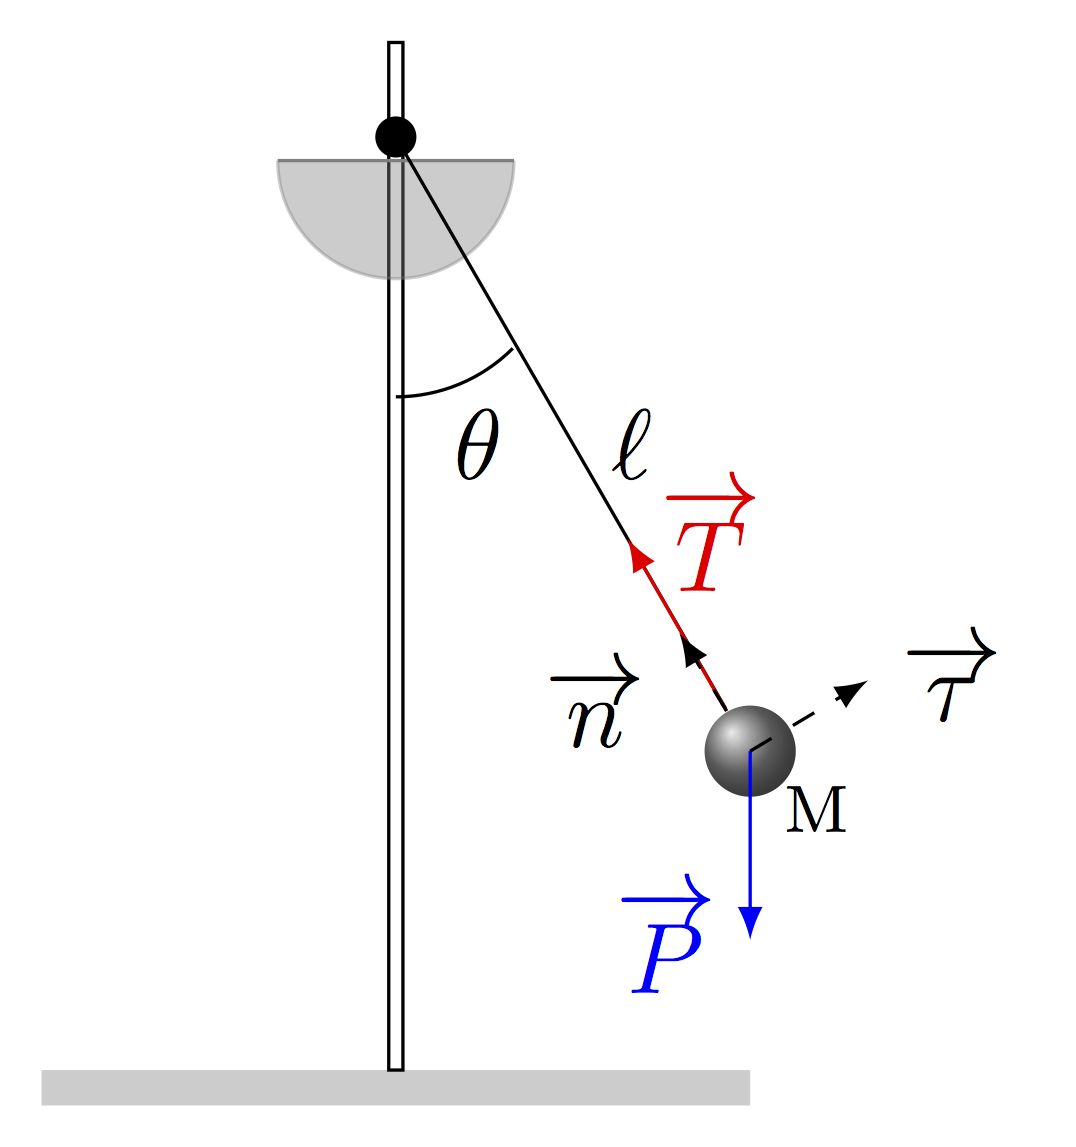
\includegraphics[scale=2]{images/modele_pendule}
	\caption{Modèle du pendule simple}
	\label{model_pendule}
\end{figure}\\
Apres application du principe fondamental de la dynamique, il vient l'équation suivante: 
\begin{equation}
	\frac{d^2\theta}{dt^2} + \frac{g}{l}\sin(\theta)=0
\end{equation}

\subsection{Simulation}
Nous avons réalisé puis simulé un modèle dans Simulink. Le pendule ne fait qu'osciller autour de 0, sa position d'équilibre car il n'y a ni frottements ni contrôle appliqué au mobile.
\begin{figure}[h!]
	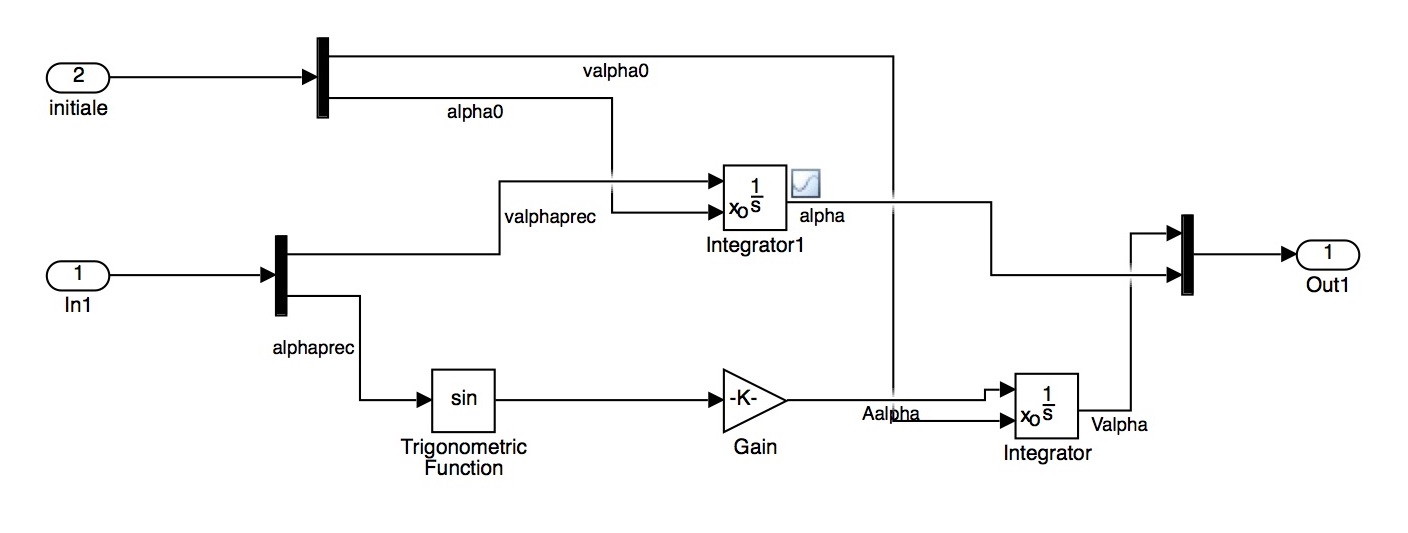
\includegraphics[scale=0.3]{images/pendule_simple_sys}
	\caption{Modèle Simulink du pendule simple}
	\label{model_pendule_simu}
\end{figure}
\begin{figure}[h!]
	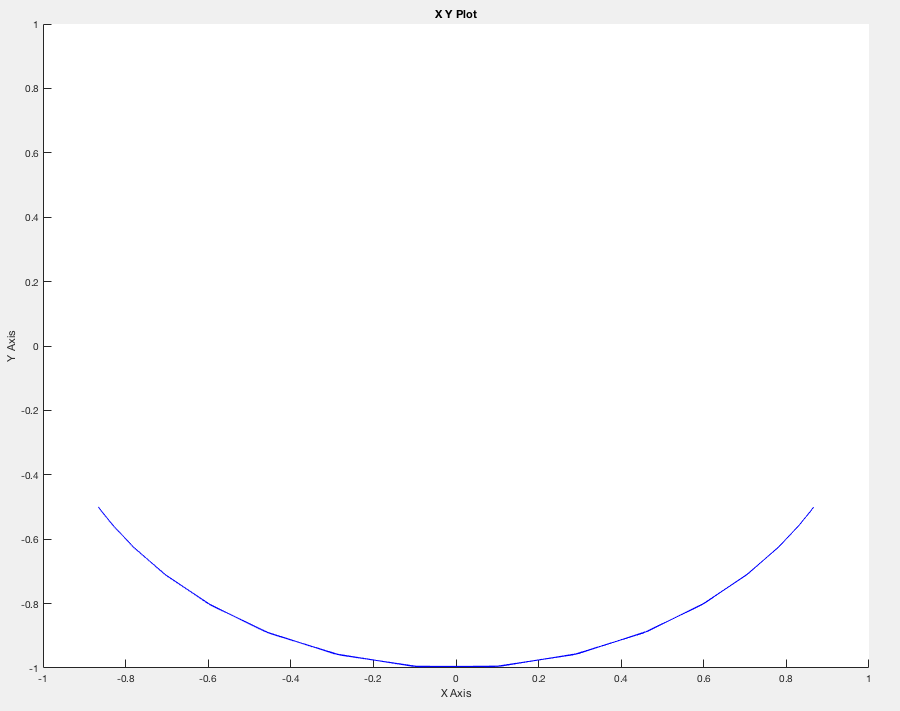
\includegraphics[scale=0.3]{images/pendule_simple_XY}
	\caption{Position du pendule}
	\label{simu_pendule_xy}
\end{figure} 
\begin{figure}[h]
	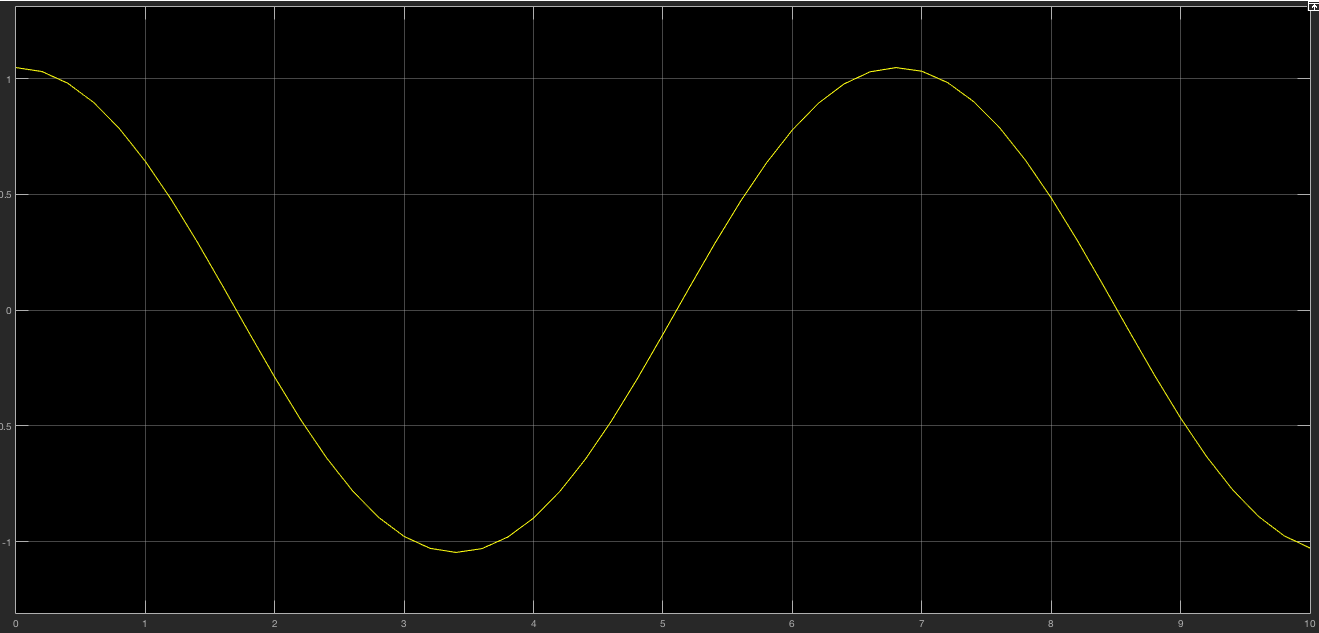
\includegraphics[scale=0.3]{images/pendule_simple_graph}
	\caption{Evolution de $\theta$ au cours du temps}
	\label{simu_pendule}
\end{figure}\\
\section{Le pendule inversé avec contrôle par une force}
\subsection{Modélisation} 
Le pendule devient inversé et un contrôle par une force est rajouté au système:
\begin{equation}
	\frac{d^2\theta}{dt} = \frac{g}{l}\sin(\theta)-\frac{u}{l}\cos(\frac{d\theta}{dt})
\end{equation}
$u$, le contrôle correspond à:
\begin{equation}
	u=u_e+K(x-x_e)
\end{equation}
Le facteur K permet a stabiliser le pendule. Sa valeur dépend de la condition initiale, plus l'angle de départ sera important plus il sera difficile de ramener le pendule à sa position d'équilibre, et il faudra un K important. K correspond à $[K_1 K_2]$, $K_1$ permet de corriger la position du mobile afin de le ramener à l'équilibre, alors que $K_2$ correspond à la vitesse ou le pendule se stabilise. En pratique ces deux facteurs sont limités matériellement, il n'est donc pas possible de leur imposer des valeurs trop importantes. \\
Ensuite nous introduirons une perturbation afin de tester la robustesse du contrôle.
\subsection{Simulation}
\begin{figure}[h!]
	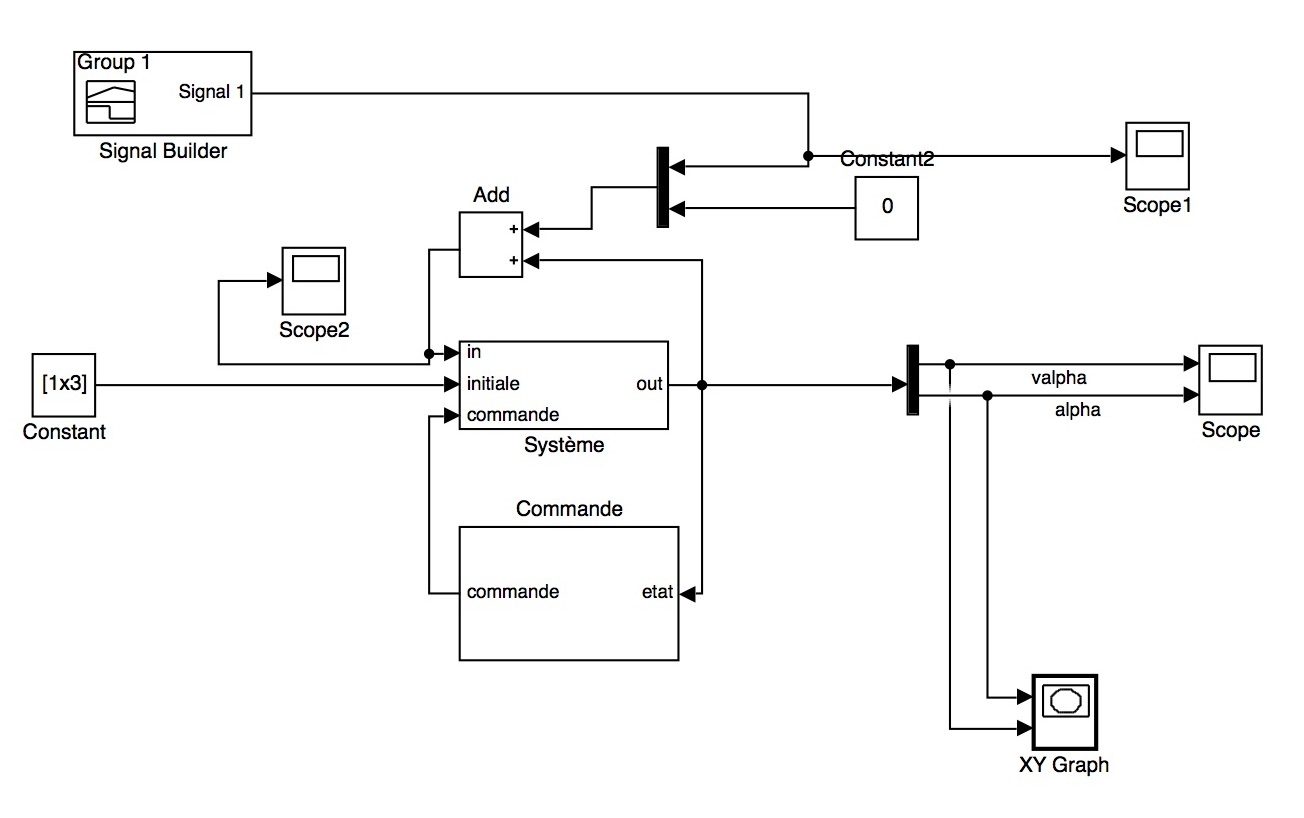
\includegraphics[scale=0.2]{images/pendule_inverse_1}
	\caption{Vue globale du système}
\end{figure}
\begin{figure}[h!]
	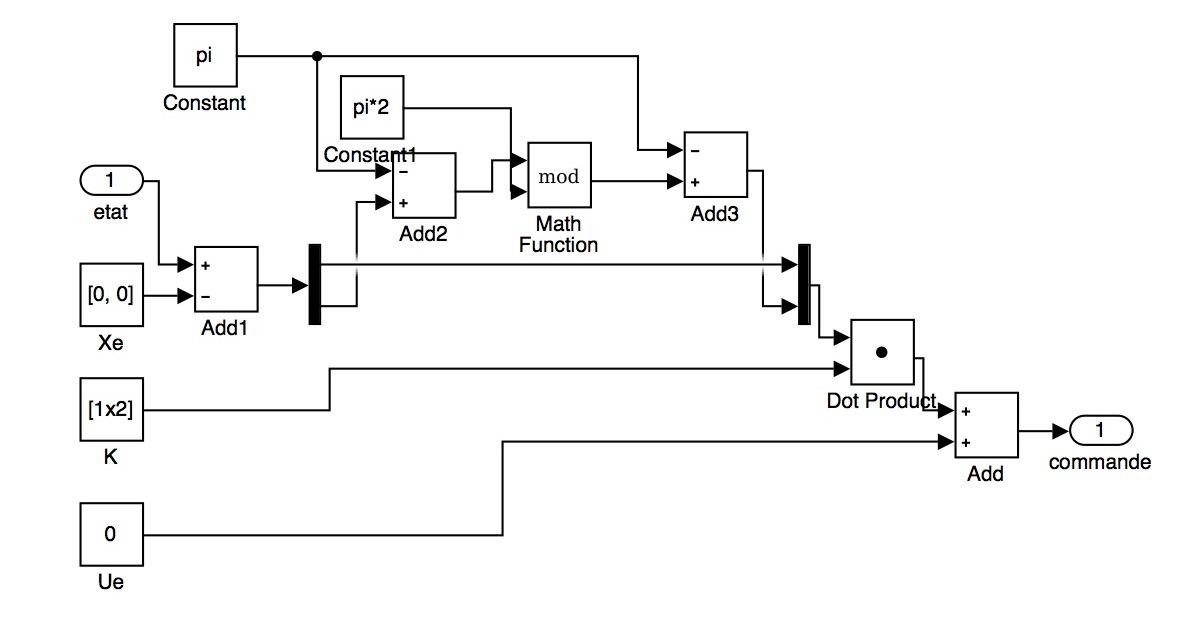
\includegraphics[scale=0.2]{images/pendule_inverse_2}
	\caption{Système de contrôle}
\end{figure}
\begin{figure}[h!]
	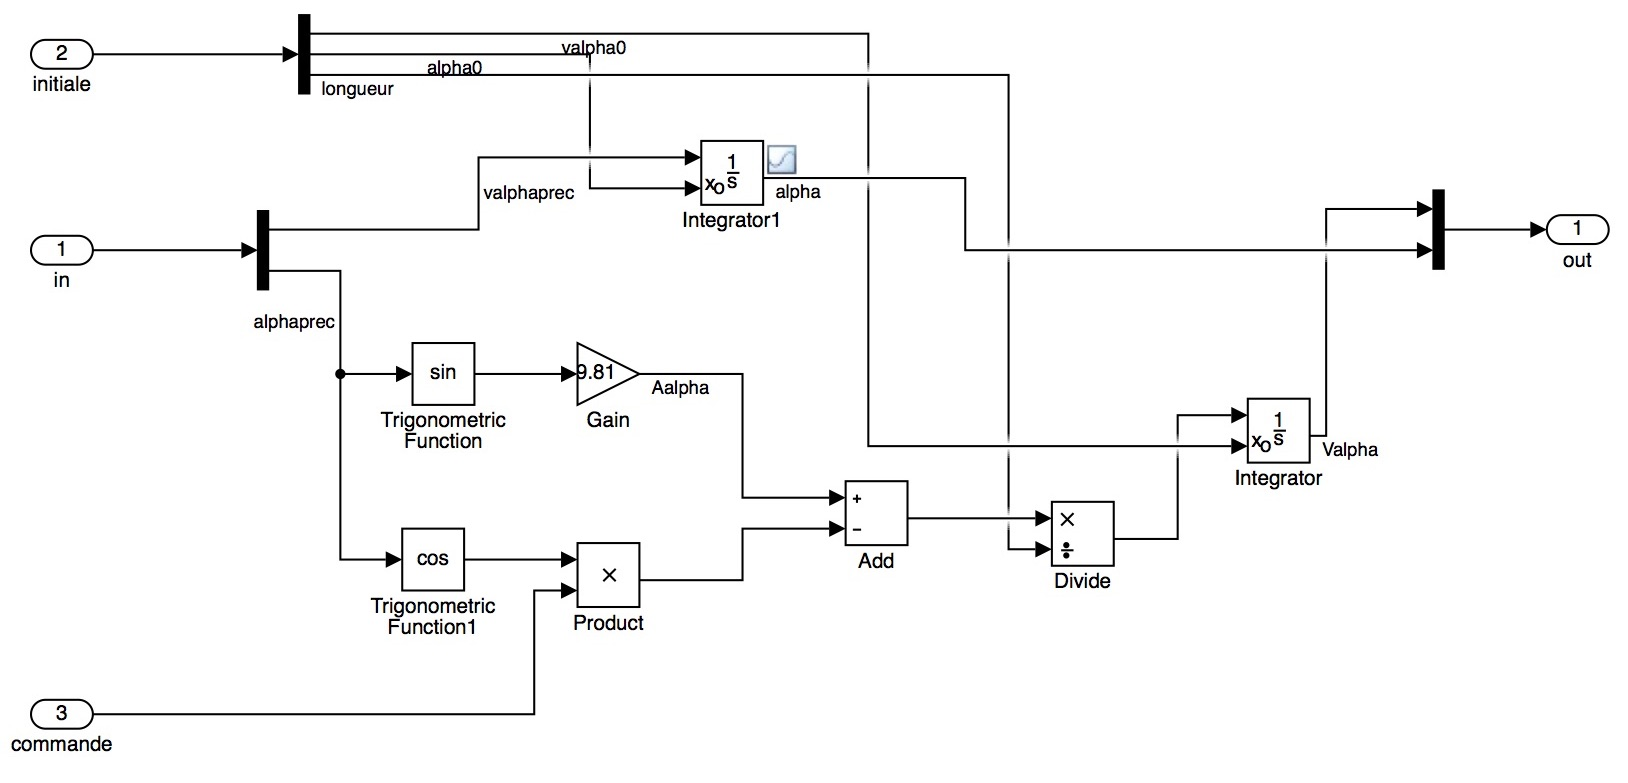
\includegraphics[scale=0.2]{images/pendule_inverse_3}
	\caption{Système}
\end{figure}
\begin{figure}[h!]
	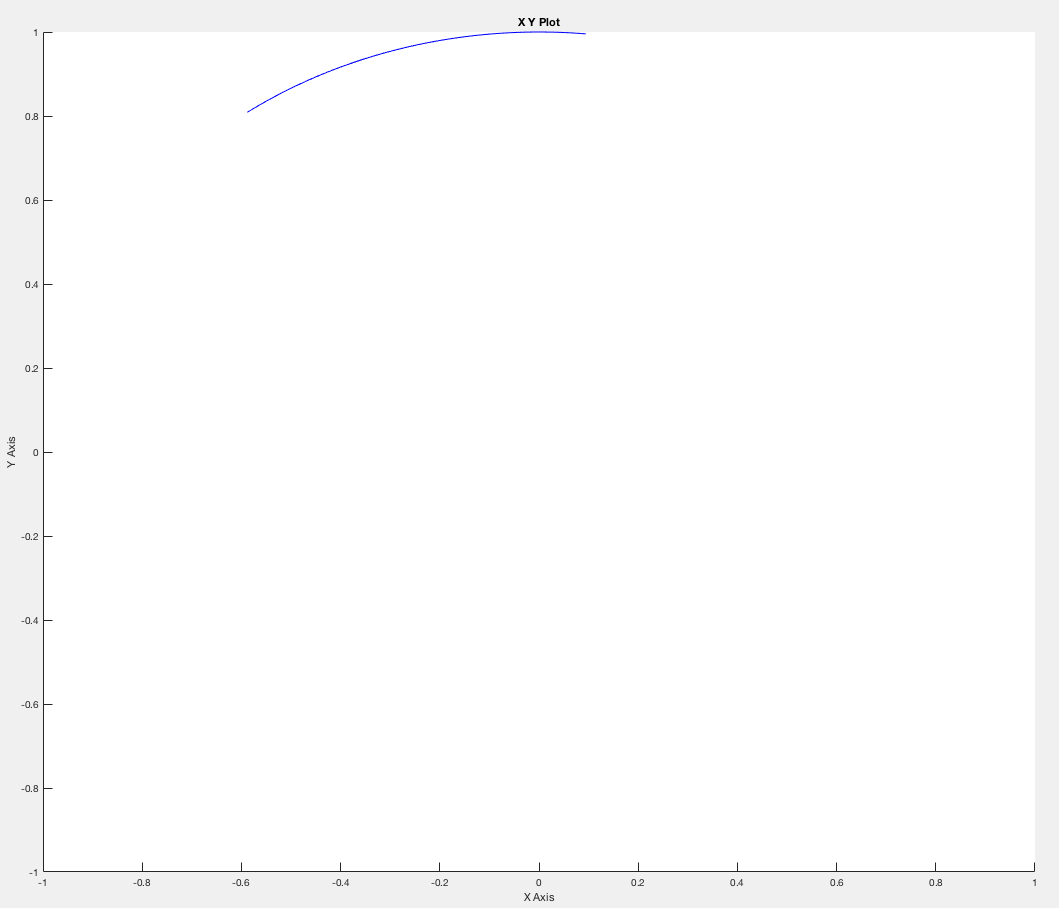
\includegraphics[scale=0.2]{images/pendule_inverse_xy}
	\caption{Position du mobile au cours du temps}
\end{figure}
\begin{figure}[h!]
	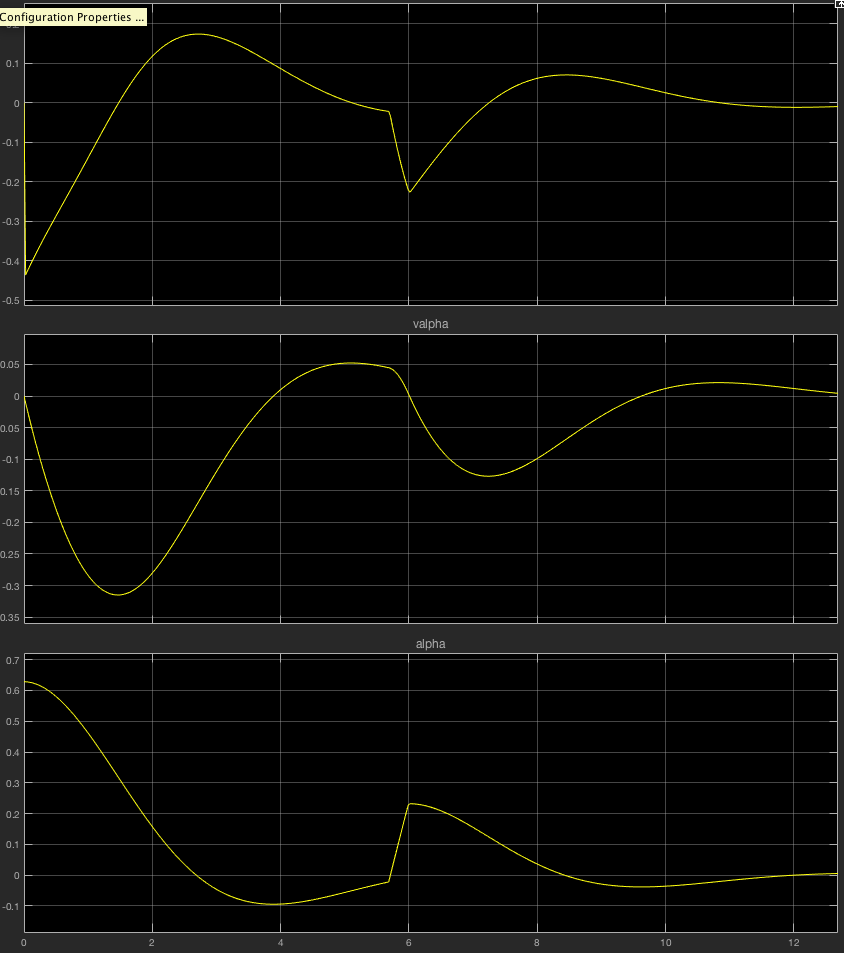
\includegraphics[scale=0.25]{images/pendule_inverse_graph}
	\caption{Variation de l'angle, au cours du temps.}
\end{figure}
\begin{figure}[h!]
	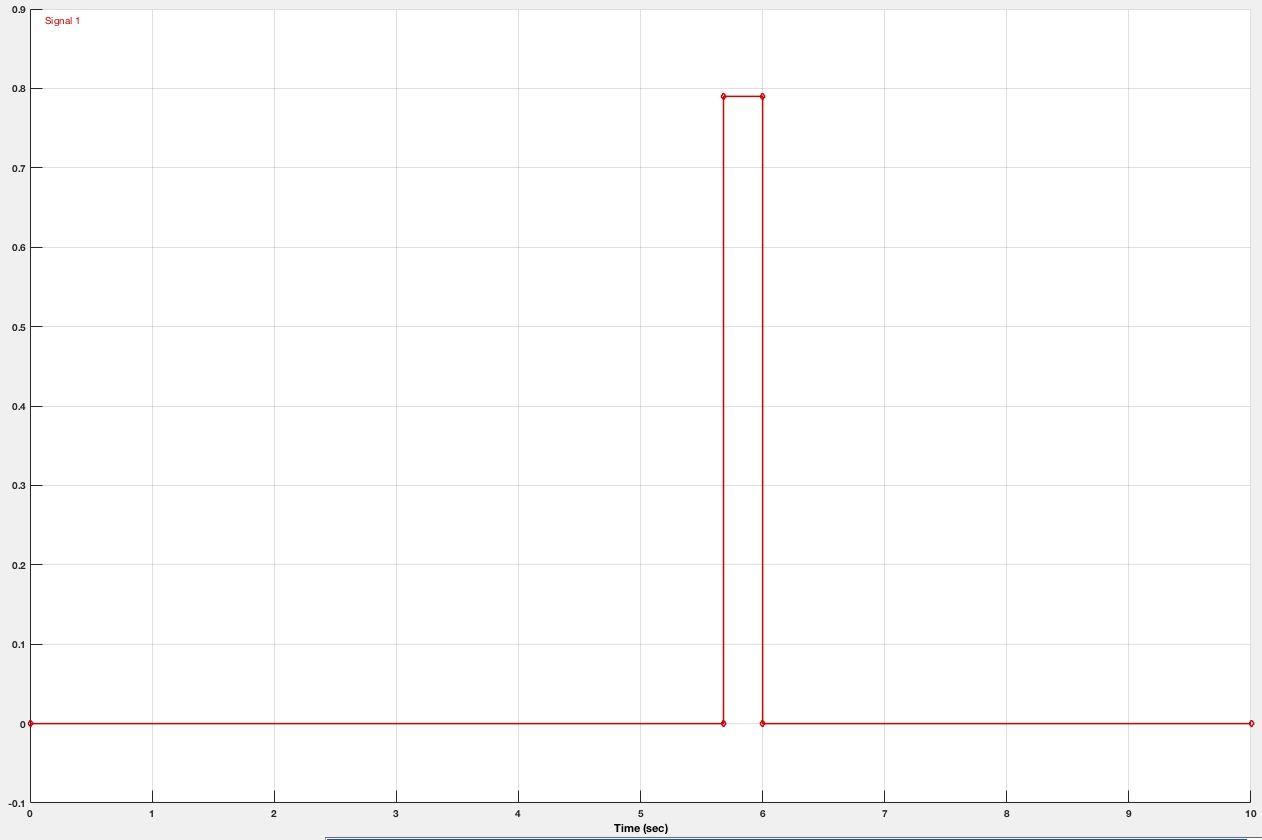
\includegraphics[scale=0.2]{images/pendule_inverse_perturbation}
	\caption{Echelon de pertubation}
\end{figure}
\section{Modèle continu et discret du robot Lego}
\subsection{Modélisation}
Le but de cette partie est de se placer au plus près de la réalité du Lego. Nous réalisons donc une modélisation et simulation discrète. Afin de reproduire le fonctionnement du Lego, nous introduisons des capteurs et prédicteurs. En effet sur le Lego nous n'avons pas accès à toute les valeurs, le robot etant équipé d'un gyroscope mesurant la vitesse de changement d'angle du pendule $\frac{d\alpha}{dt}$, il faut donc reconstruire les autres valeurs a l'aide d'un sous-sytème prédicteur.
\subsection{Simulation}

\section{Application embarquée dans le robot Lego}

Le but final du projet est d'implémenter le modèle simulé sous simulink dans le robot Lego et de le faire tenir à la verticale. Le robot fournie la vitesse de variation de l'angle verticale($d\psi$) et la position de la roue ($\theta_m$). Comme dans la simulation, on réalise alors un prédicteur avec un intégrateur et dérivateur discret. On fixe ensuite une commande K calculée avec des valeurs propres négatives.

Une fois le programme uploadé et lancé le robot, le robot commence à osciller avant de sortir de la zone de contrôle. Cette perte de contrôle est surement dû à un mauvais choix de K. En effet, même si le K choisi possède des valeurs propres négatives, on n'émet aucune propriété sur la vitesse de convergence et d'hypothèse de convergence dans un cas discret. Certains K pourraient donc s'avérer plus adéquat pour des intégrateurs discret avec une modélisation réaliste que dans un certain domaine de variation.

\section*{Conclusion}
\end{document}